 % !TeX root = ../main.tex
\chapter{Parking Detection}\label{chapter:Parking Space Detection}
First step in \acrfull{ap} is to find a parking vacancy. This step is really important and could be the base step in parking scenario because it parking maneuver could be affected by that. For example if there is not enough space, parking maneuver would not be successful. Hence, in this research many times and efforts have been taken to find a best method of parking space detection. Various approaches has been presented for parking vacancy detection in recent years. We selected vision method and \acrlong{ml} methods for parking detection. Some \acrshort{ml} and \acrshort{nn} methods have been also presented previously, among which we could point ti \cite{histogramEOH}. In\cite{histogramEOH} orientation histogram and density computation were used to identify empty parking lot. As it's mentioned in \ref{chapter:related_wrok}, many of the vision based methods uses parking space line markers in street and garages to define different parking areas and marking points as in\cite{markingPointJournal}marking points are defined as edges of each parking area and after finding this point it would be easier to find a free area for parking. One of the problem which is addressed about vision ways is that they always need to have visual based data of parking-lot to make decision of parking occupancy otherwise it is more reliable method than sensor because although sensors would provide precise data of distances and measurements, they could not process other information of the scene as position of vehicle, object detection and they just consider cars as data and other features would be ignored. 
In this work, a simple vision base method has been used. At first, vehicles in front of the ego vehicle should be detected and then based on vehicles' positions and sizes and comparing them to the main(ego) vehicle, free parking place would be detected.
\section{Vehicle Detection}\label{vehicle detection}
The idea is to detect cars in front of the ego vehicle and based on the distance between first two vehicles ahead, parking space would be detected. Detection is based on the images taken by camera-sensor. Camera sensor is placed in front of the ego vehicle and during simulation while vehicle passes the street, images from side of the street are captured and sent to the detection algorithm. The goal is to detect vehicles in images so it is a textbox object detection problem.  As it mentioned in \ref{chapter:Background}, lots of machine learning algorithms could be used to detect object in an image. The most common ones are as follows:
\begin{itemize}
\item \textbf{\acrfull{hog}}
 \item \textbf{\acrlong{cnn}}
 \item \textbf{\acrshort{rcnn}, FastRCNN and Faster-RCNN}
 \item \textbf{\acrshort{yolo}}
 \item \textbf{\acrshort{acf}}
\end{itemize}
In this thesis, three detectors were trained(two detectors from FasterRCNN by setting different training parameters and one detector from ACF method) and finally ACFObjectDetector was selected as our vehicle detection algorithm because it provided more accurate detection on our specific training data. Despite our expectation that RCNN would provide better result because of its popularity, detector from ACF worked better in our training data. Another reason could be referred to the training dataset as FasterRCNN requires a specific training dataset. Since the results of ACFObjectDetector were more satisfied and this method was working better in our data, ACF detector has been selected and working on better algorithm for training FasterRCNN postponed to future works. Next section presents an explanation of the methods which have been used. Evaluation results from the detector of each method after training step, has been also provided.
\subsection{FasterRCNN}
At first test, 656 labeled images(results of groundTruth labeler) fed into the network in learning process and Epochs set to be 40 as it supposed to provide a more accurate data by training with more epochs and learning iterations. However, if these epochs number exceeded certain values, network would be over-trained. 40 epochs resulted in 26240 iteration for each step of training (as RCNN has 4 training steps) and accuracy rate for each step was closed to 98-100 percent. Fig \ref{fig:40E_training} illustrates a moment of training process in the last training step.
\begin{figure}
    \centering
     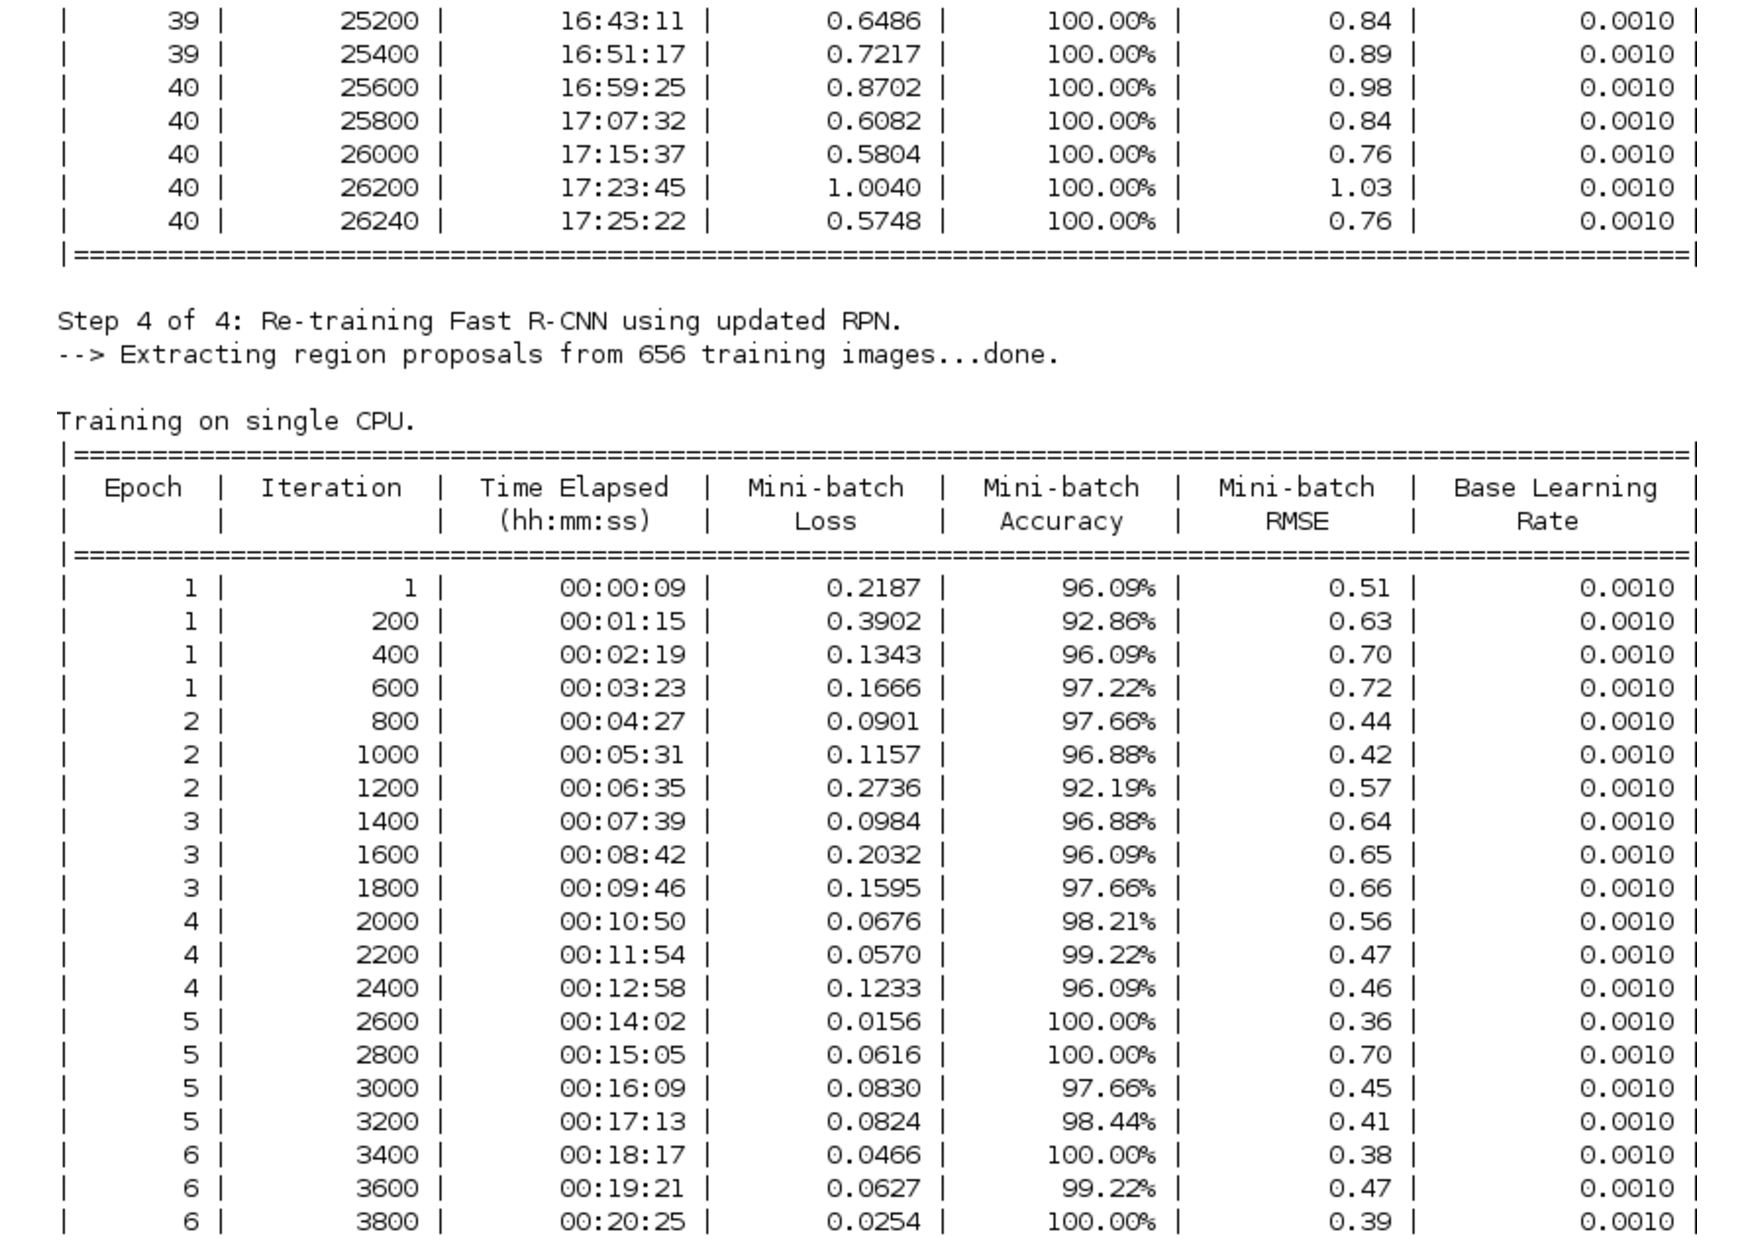
\includegraphics[width=14cm, height=8cm]{images/rcnn40E.pdf}
     \caption{FasterRCNN Training Process - Set to 40 Epochs }
     \label{fig:40E_training}
\end{figure}
Fig \ref{fig:rcnnVsACFResult} illustrates results of RCNN detector and ACF detector respectively(from left to right). First left image in the first was the testing image to examin results of different detectors. Second image(first row) shows detection result of FasterRCNN(trained with 40 Epochs) and it detected two of 3 vehicles. Finally, the last image in first row is the result of ACF detection where all vehicles covered with bounding boxes which means that ACF detected all of the 3 vehicles. In second row another image that includes 2 cars, has been tested and again the results of RCNN and ACF could be observed from left to right. As it can be seen, FasterRCNN detected none of the vehicles as it shows empty bboxes and empty scores(0*1 empty). Second image is the result of ACF which shows 3 detection(for 2 cars in image?) because sometimes we could get more than one detection for one vehicle and here the first 2 bboxes are for first vehicle and the second bboxes is for the other vehicle. However, in this situation where there are more than one detection for one vehicle with different scores, strongest score would be selected. Here after selecting the strongest scores by eliminating same detection(bboxes for one vehicle which have overlaps), the result of ACF is the last photo in row 2 which shows that it detected both vehicles but RCNN could not detect any of them. There was a probability that RCNN was over-trained because of 40 epochs or many repetitive training samples.
\begin{figure}
\centering
\begin{tabular}{ lccc } 
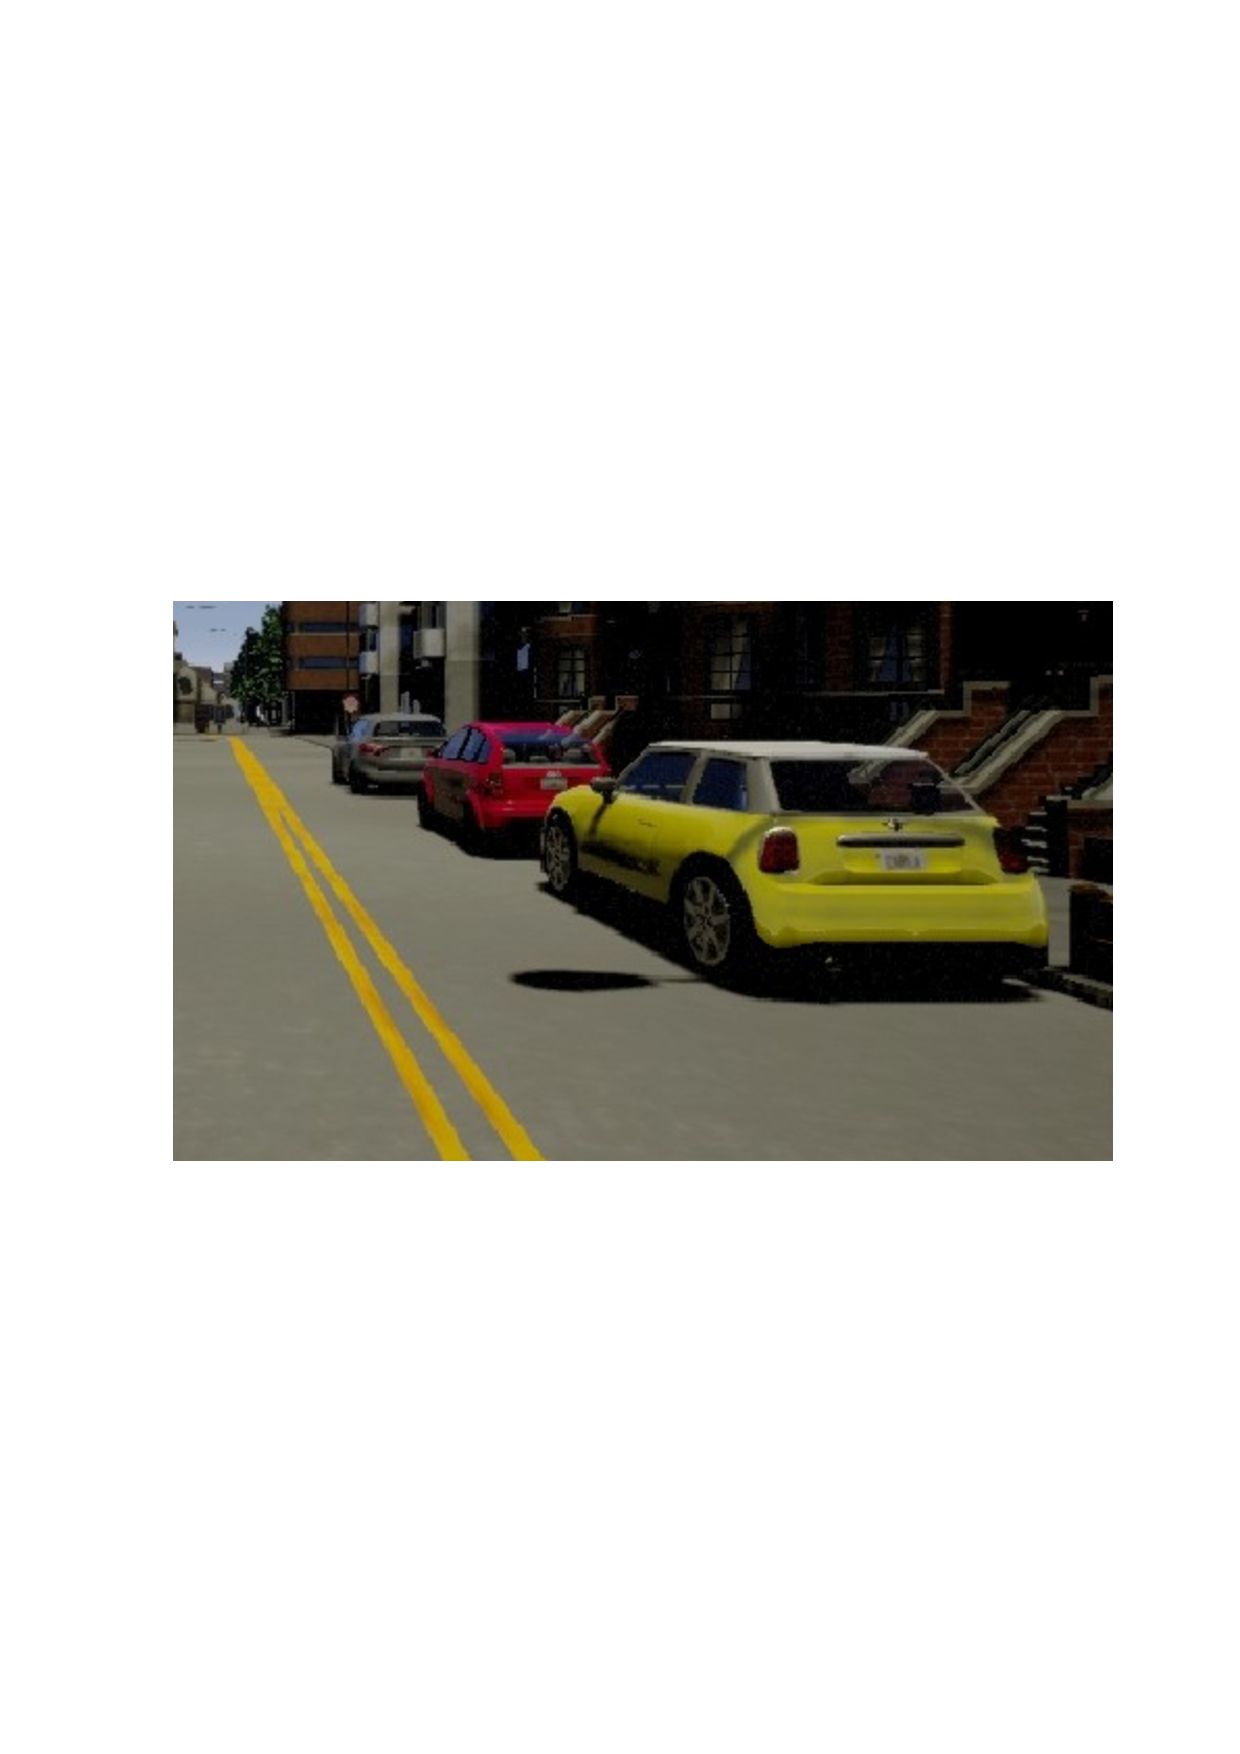
\includegraphics[width=4cm, height=6cm]{images/rawImg.pdf}
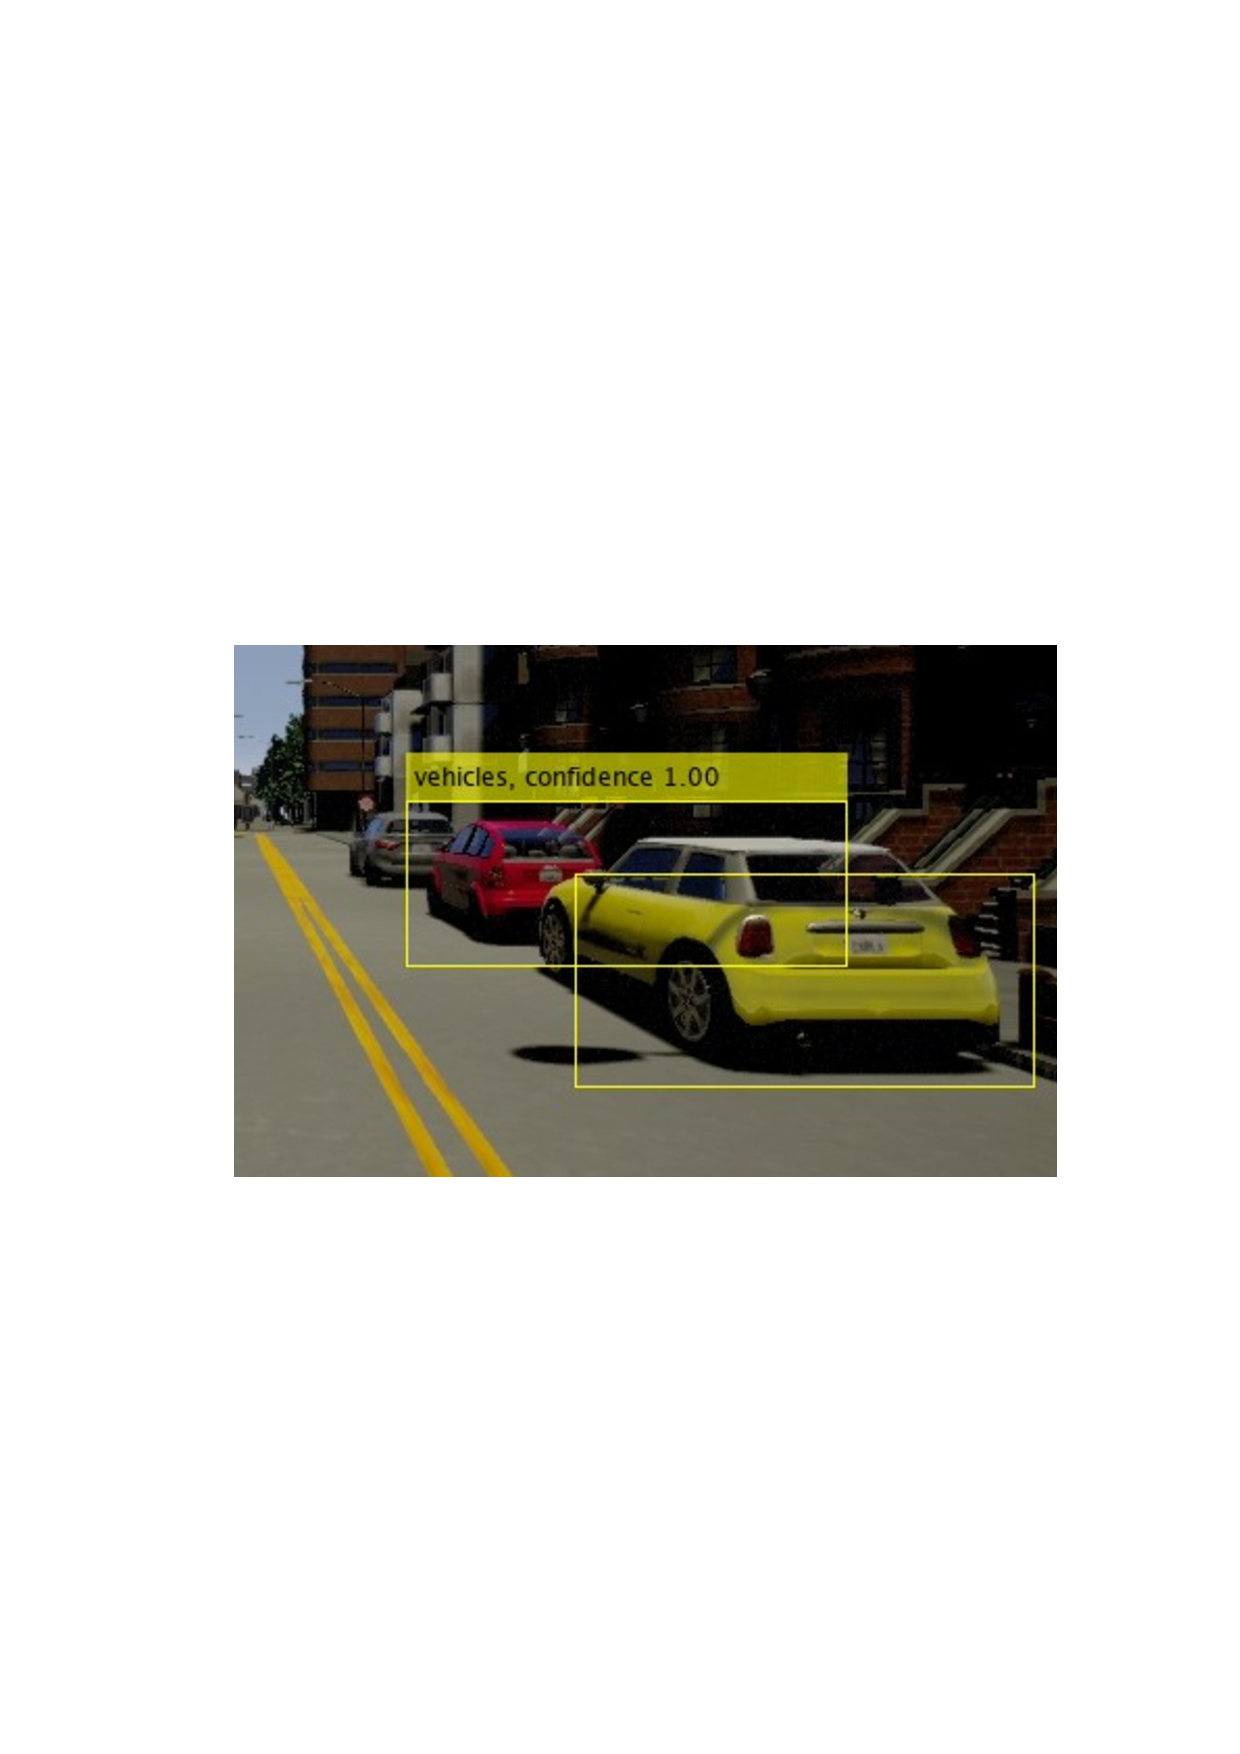
\includegraphics[width=4cm, height=6cm]{images/RCNN40.pdf} 
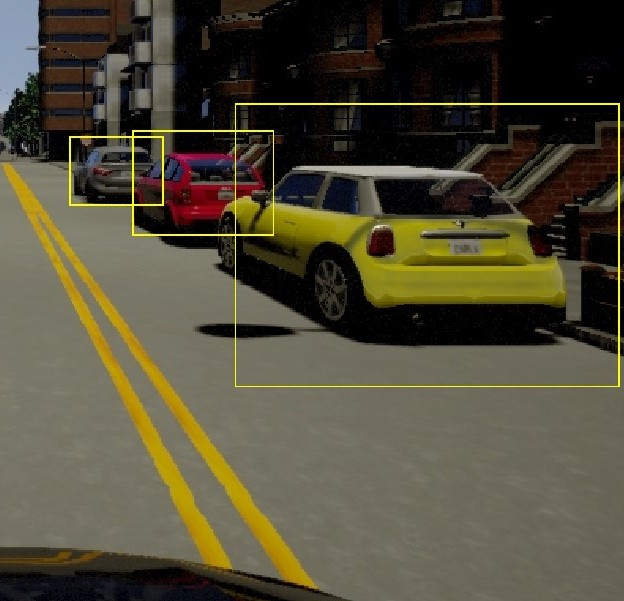
\includegraphics[width=4cm, height=6cm]{images/acf.jpg} \\ 
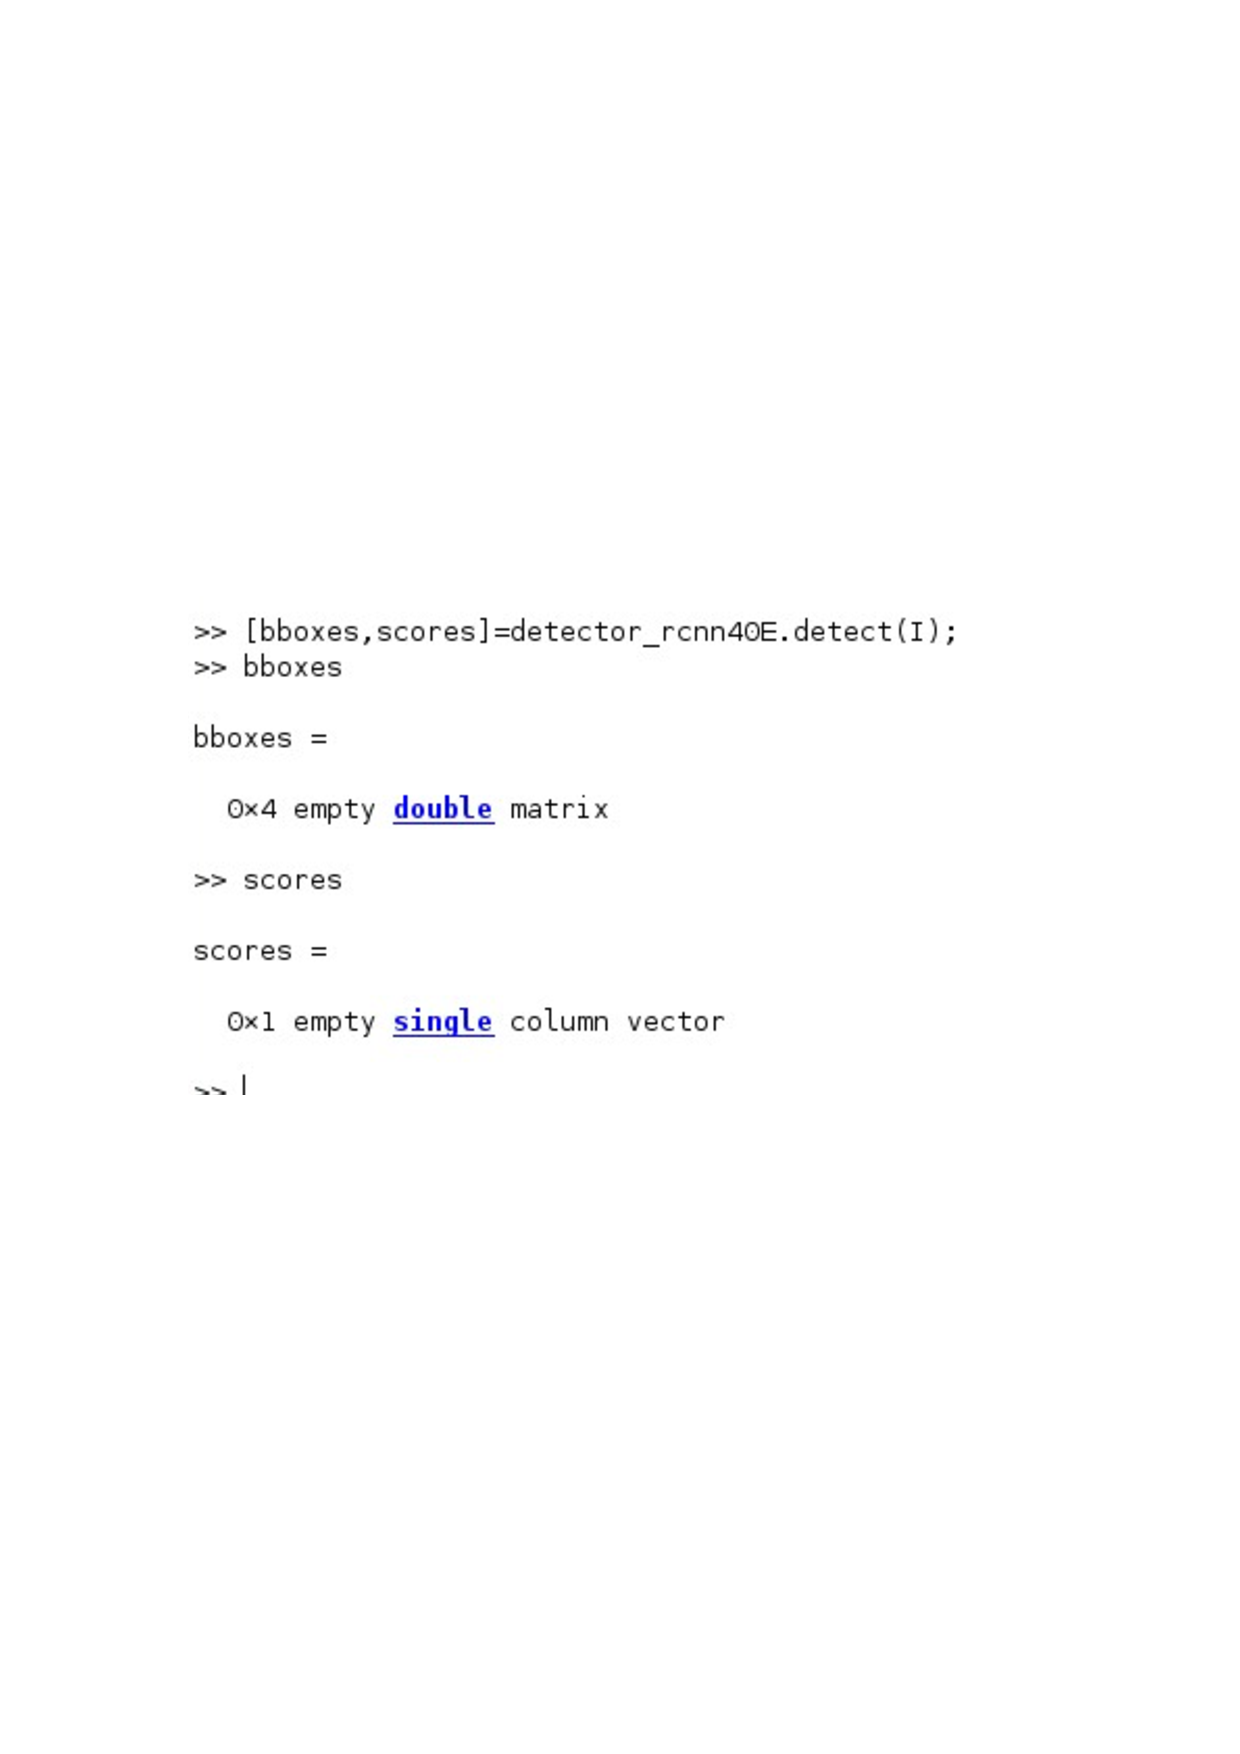
\includegraphics[width=4cm, height=5cm]{images/test4RCNN40.pdf}
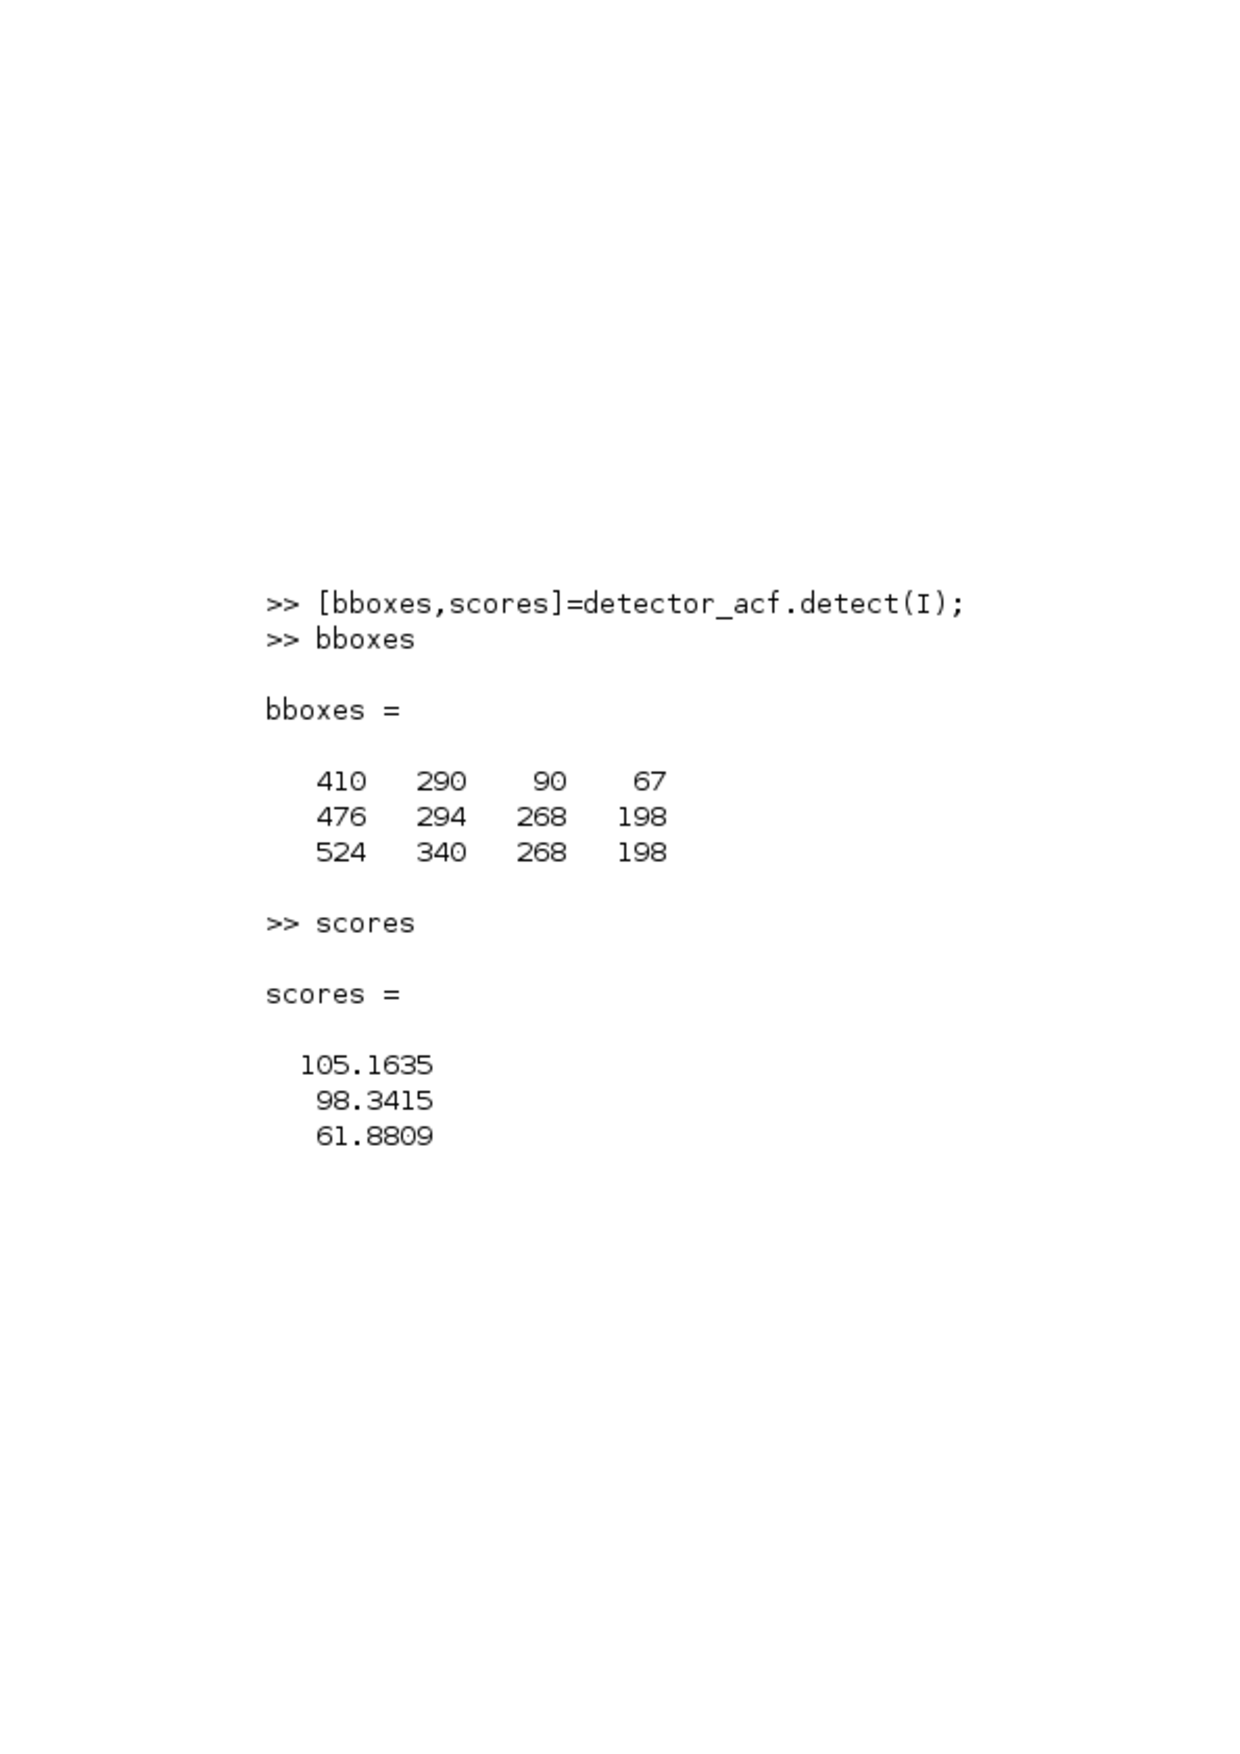
\includegraphics[width=4cm, height=5cm]{images/acfTest4.pdf} 
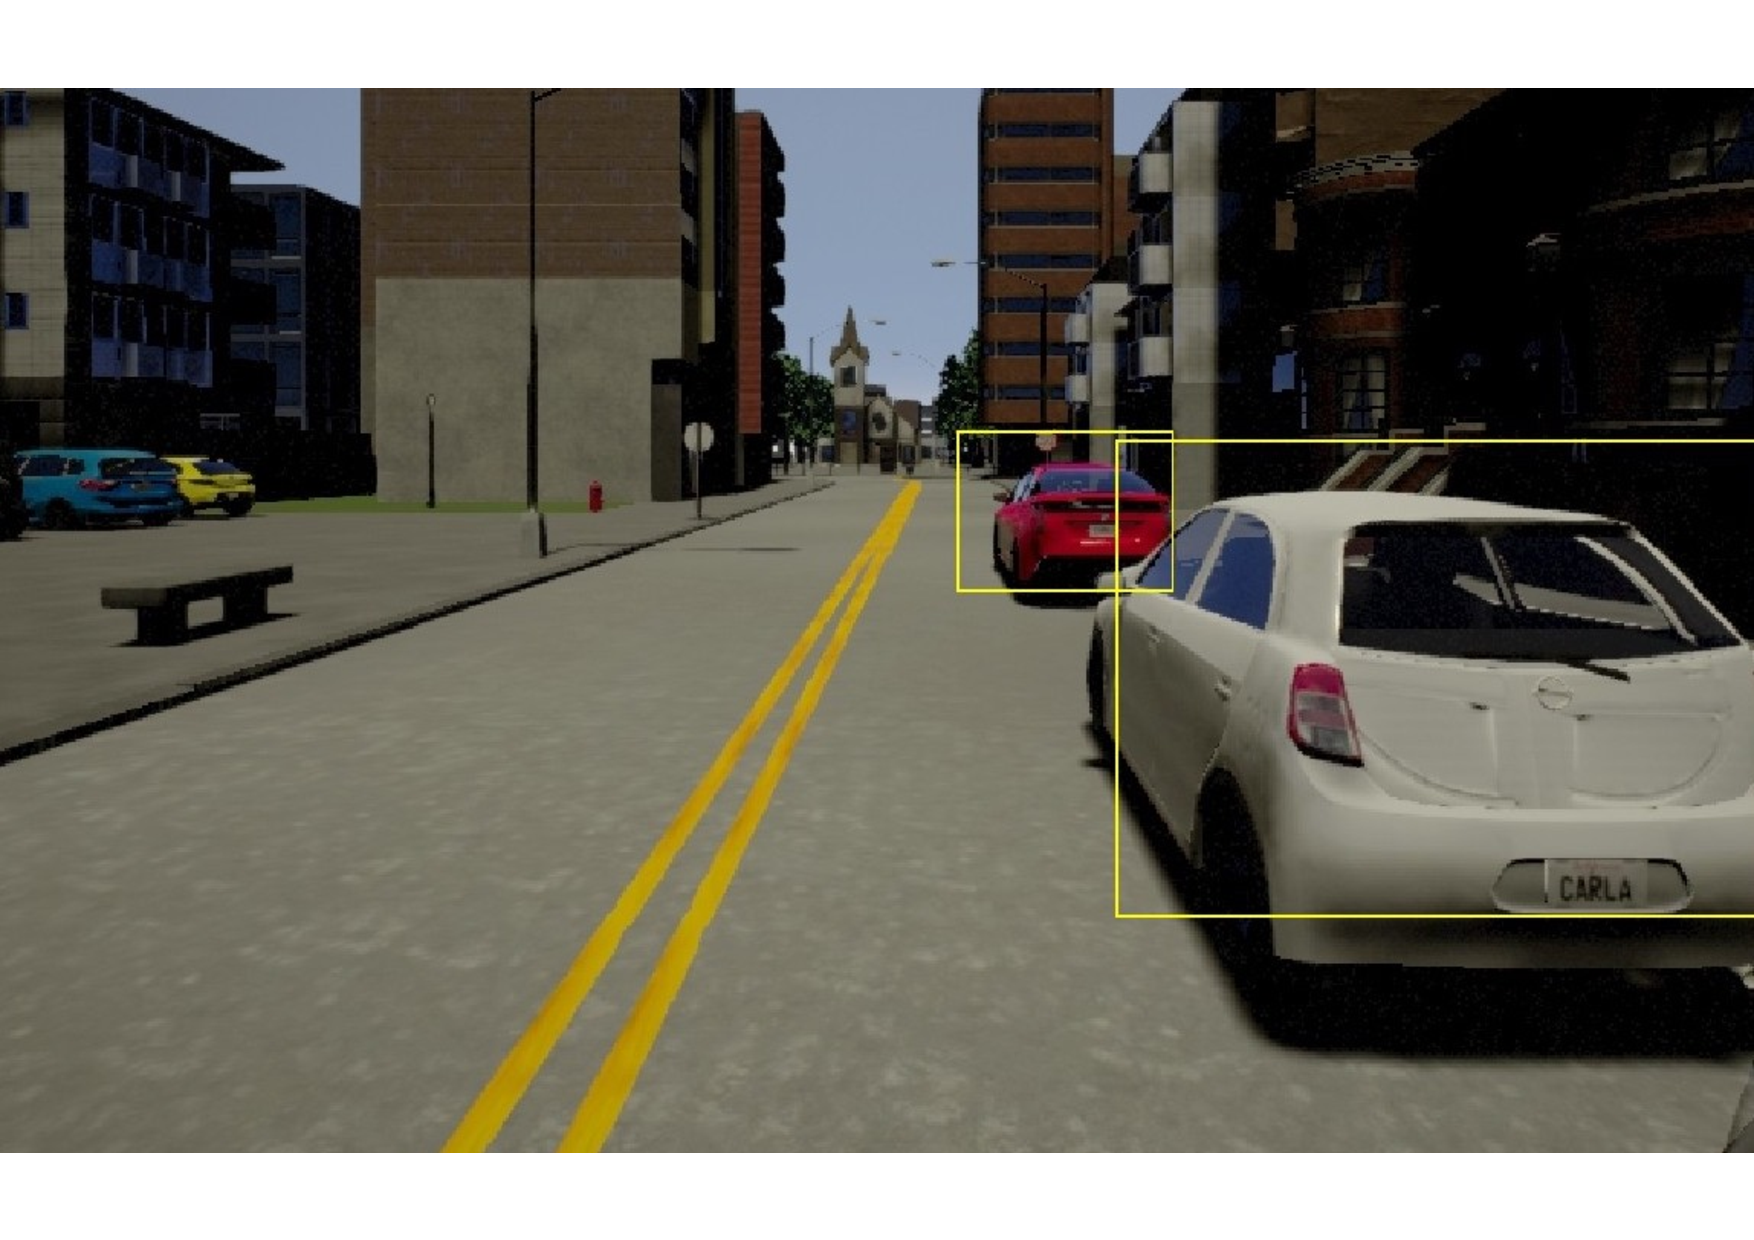
\includegraphics[width=4cm, height=5cm]{images/test4ACFview.pdf}
\end{tabular}
\caption{Detection results of ACFObjectDetector and FasterRCNN}
\label{fig:rcnnVsACFResult}
\end{figure}

So next time we decided to reduce number of repetitive data as far as possible. This time 188 images were chosen in the training step and Epochs reduced to 10 numbers so we had 1880 learning iteration in each step and accuracy rate was more than 82 as it can be seen in \ref{fig:RCNN10E}. Although the accurate rate of training was reduced compared to the last time, detection results were exactly the same as last detector(trained by 40 epochs) for same testing samples.
\begin{figure}
    %\begin{tabular}{c|c}
        % 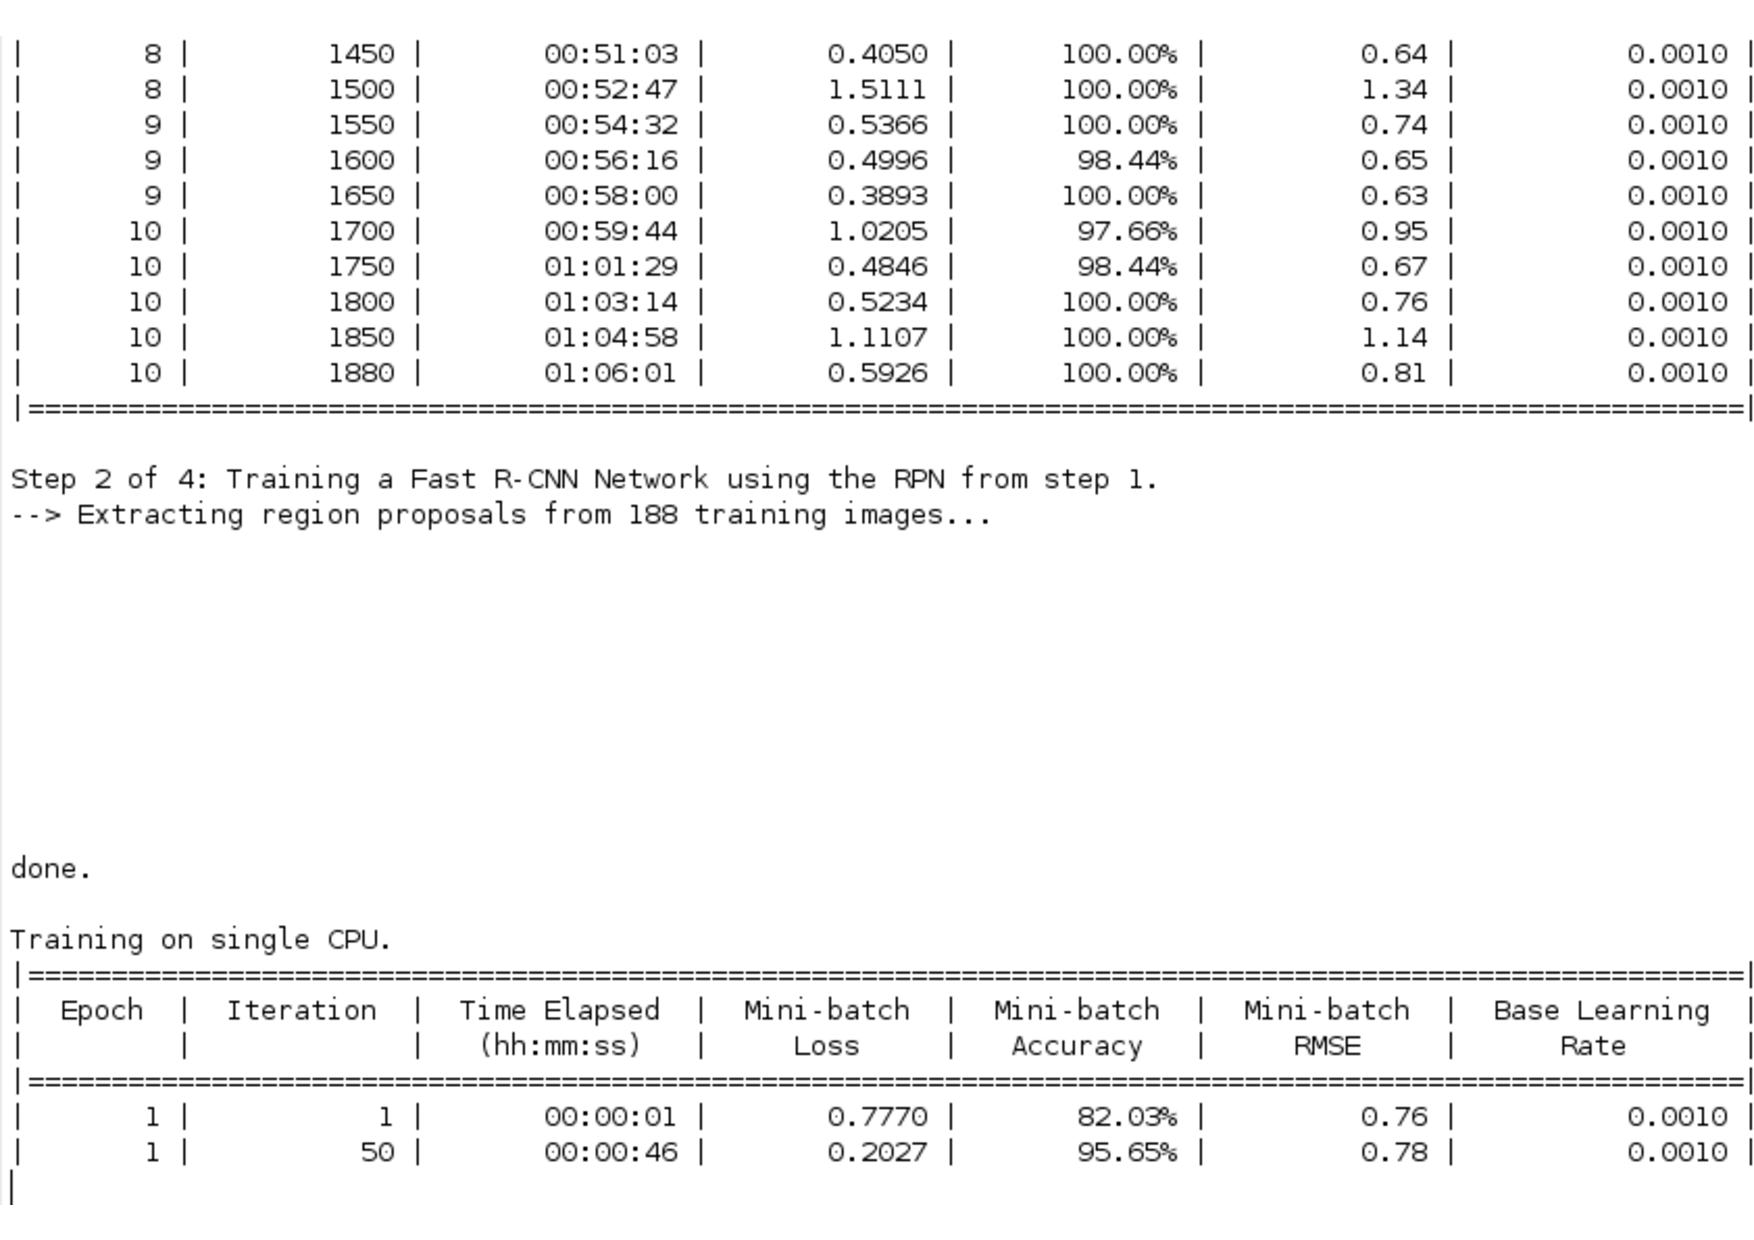
\includegraphics[width=6cm, height=8cm]{images/1.pdf} 
         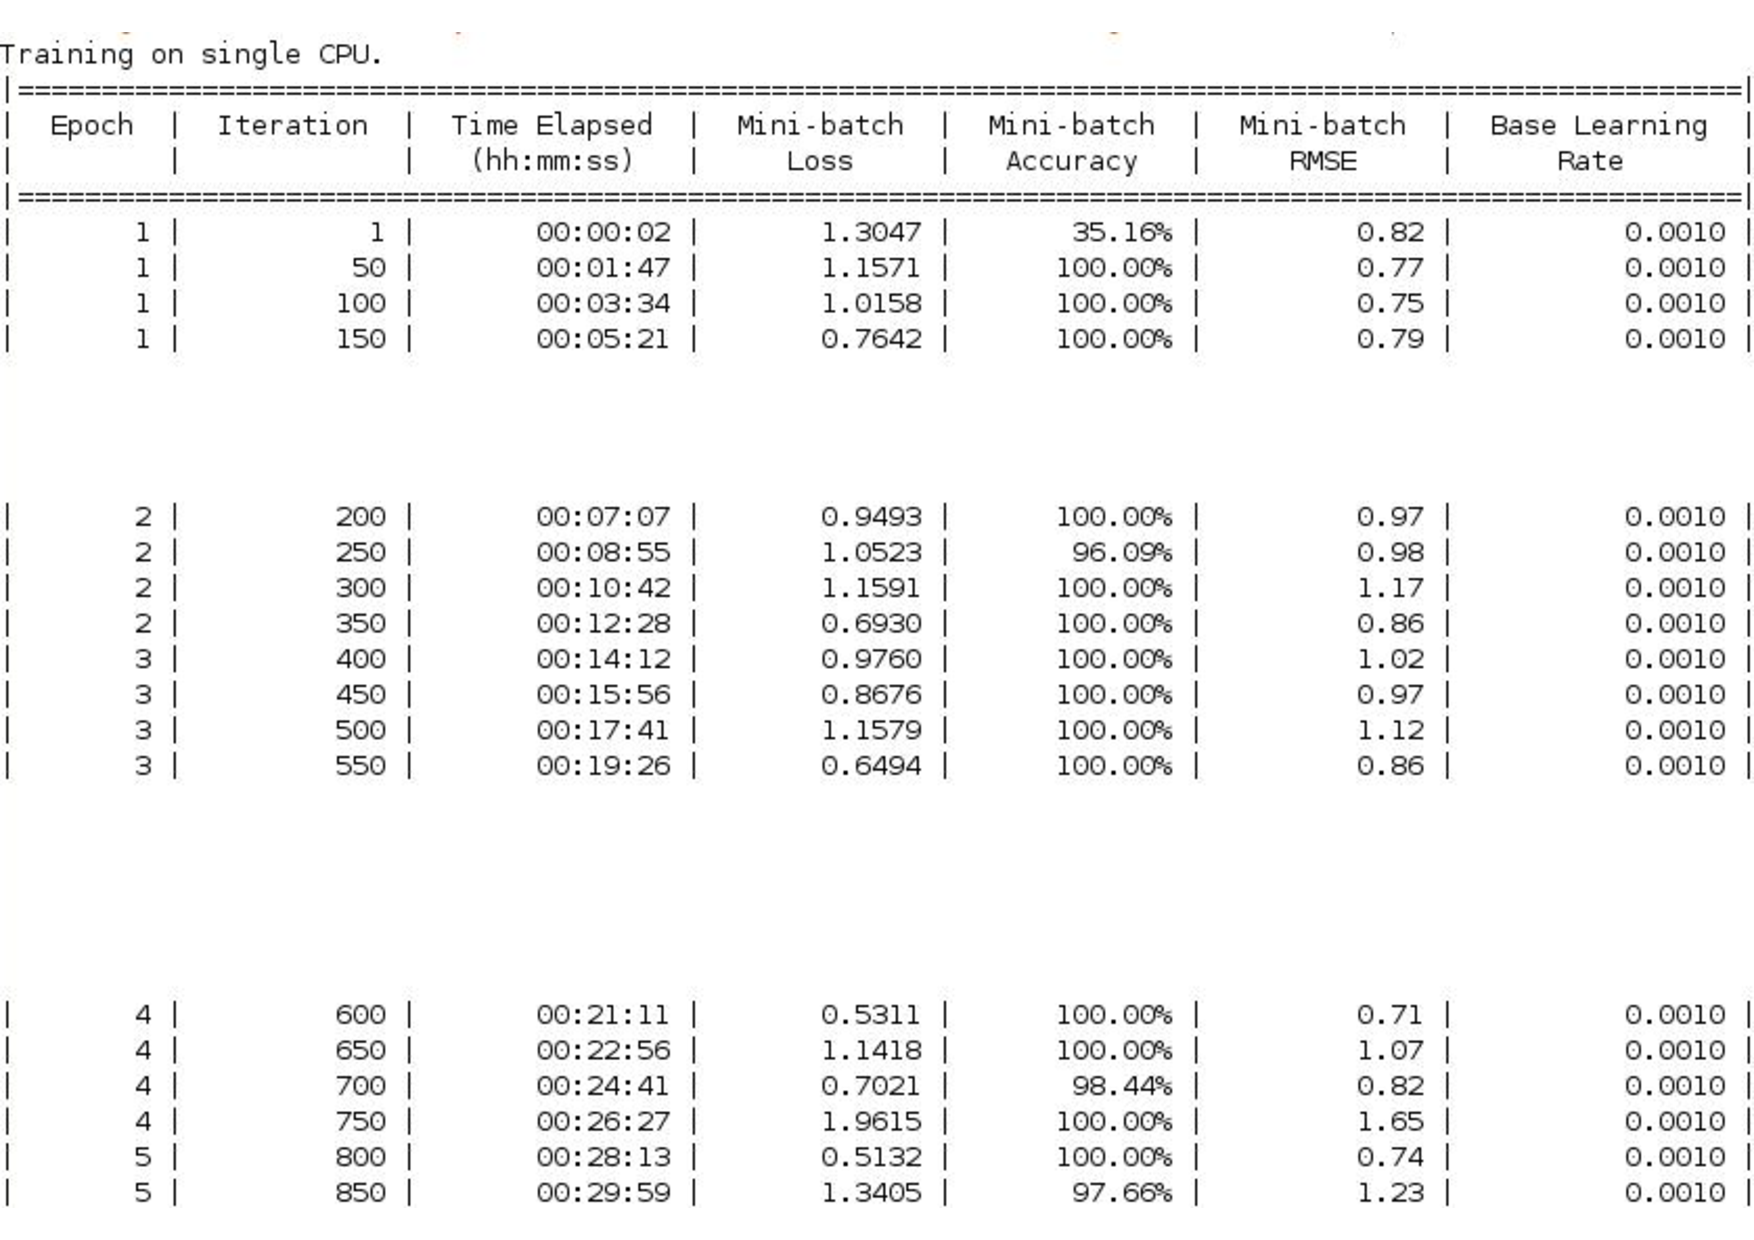
\includegraphics[width=14cm, height=8cm]{images/2.pdf}
   % \end{tabular}
    \caption{Training process of FasterRCNN with 10 epochs}
    \label{fig:RCNN10E}
\end{figure}
\subsection{ACFObjectDetector}
ACFObjectDetector with 5 training steps have been generated and same dataset from training last detector(FasterRCNN with 10 epochs) has been used to see the difference. \ref{fig:acfTrainProcess} shows a moment of ACF training. 
\begin{figure}
    \centering
    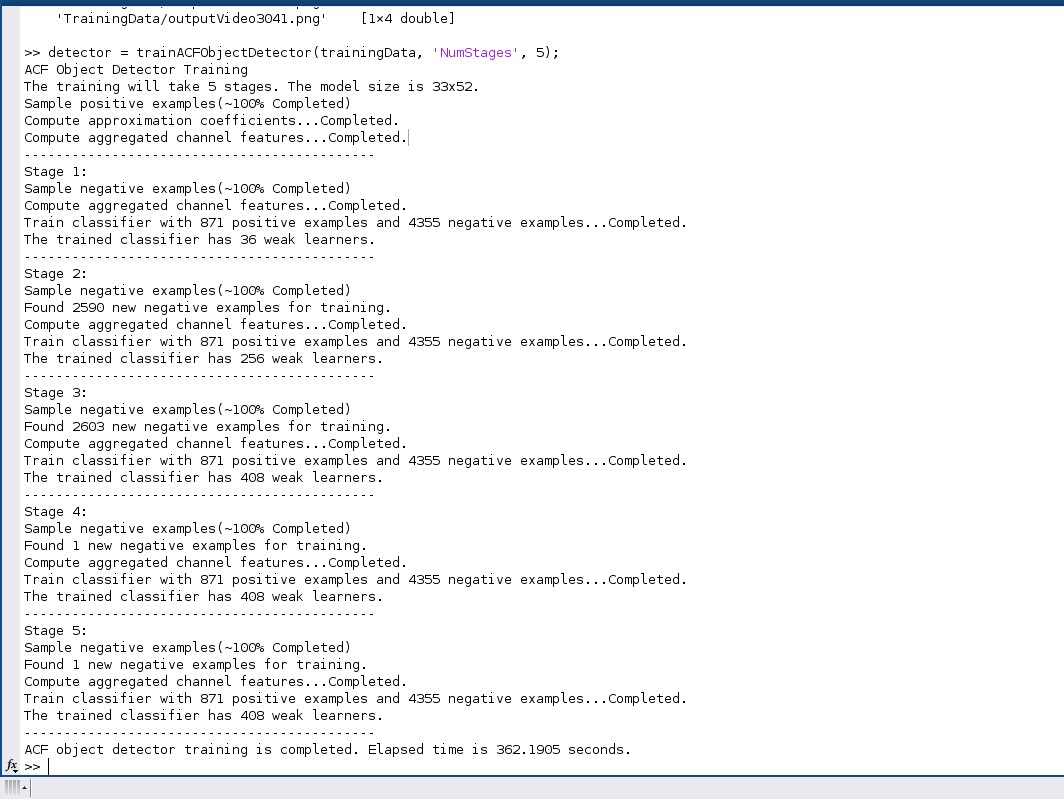
\includegraphics[width=12cm, height=8cm]{images/TrainpocessACF.jpg}
    \caption{Training ACFObjectDetector}
    \label{fig:acfTrainProcess}
\end{figure}
Evaluation results can be seen in \ref{fig:evaluation}. Same testing samples were used to measure the efficiency of three different detectors. Two \acrshort{rcnn} detectors provided the exact same precision rates of 20 percent. ACF has the better detection rate (70 percent)
\begin{figure}
\centering
    \begin{tabular}{lccc}
    \space\textbf{FasterRCNN detector - training epochs set to 10}\\
         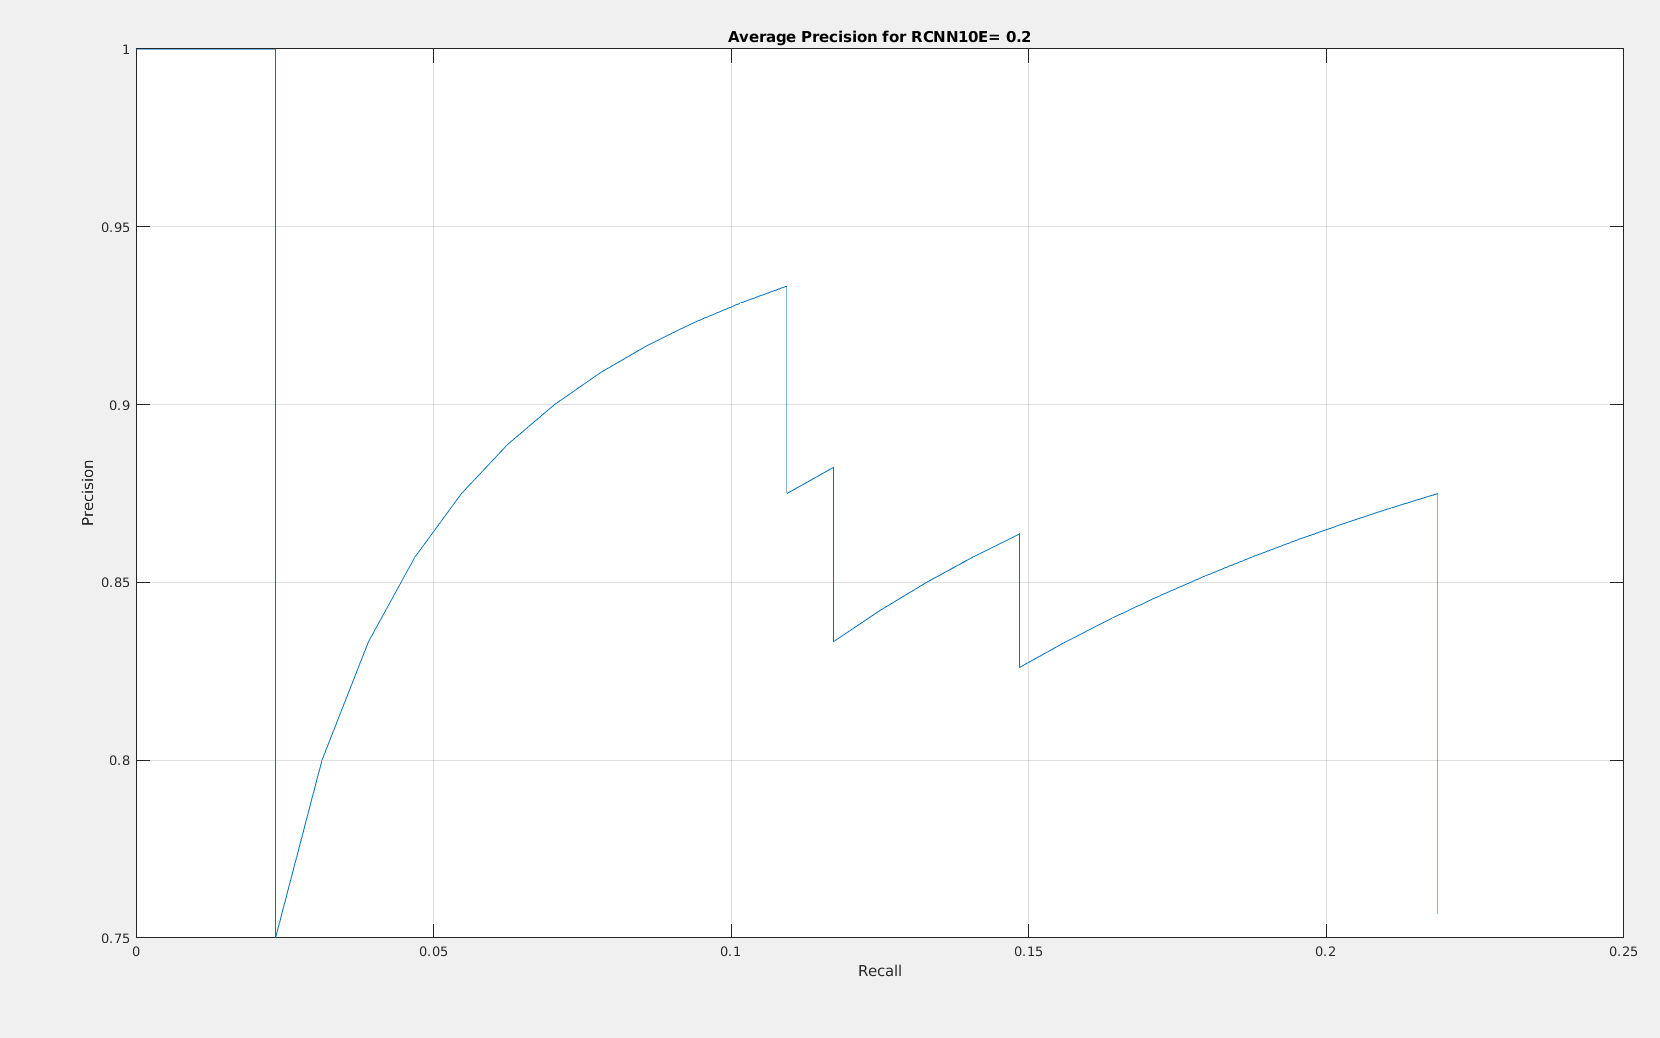
\includegraphics[width=12cm, height=5cm]{images/Evalrcnn10E.png} \\
         \space \textbf{FasterRCNN detector - training epochs set to 40}\\
         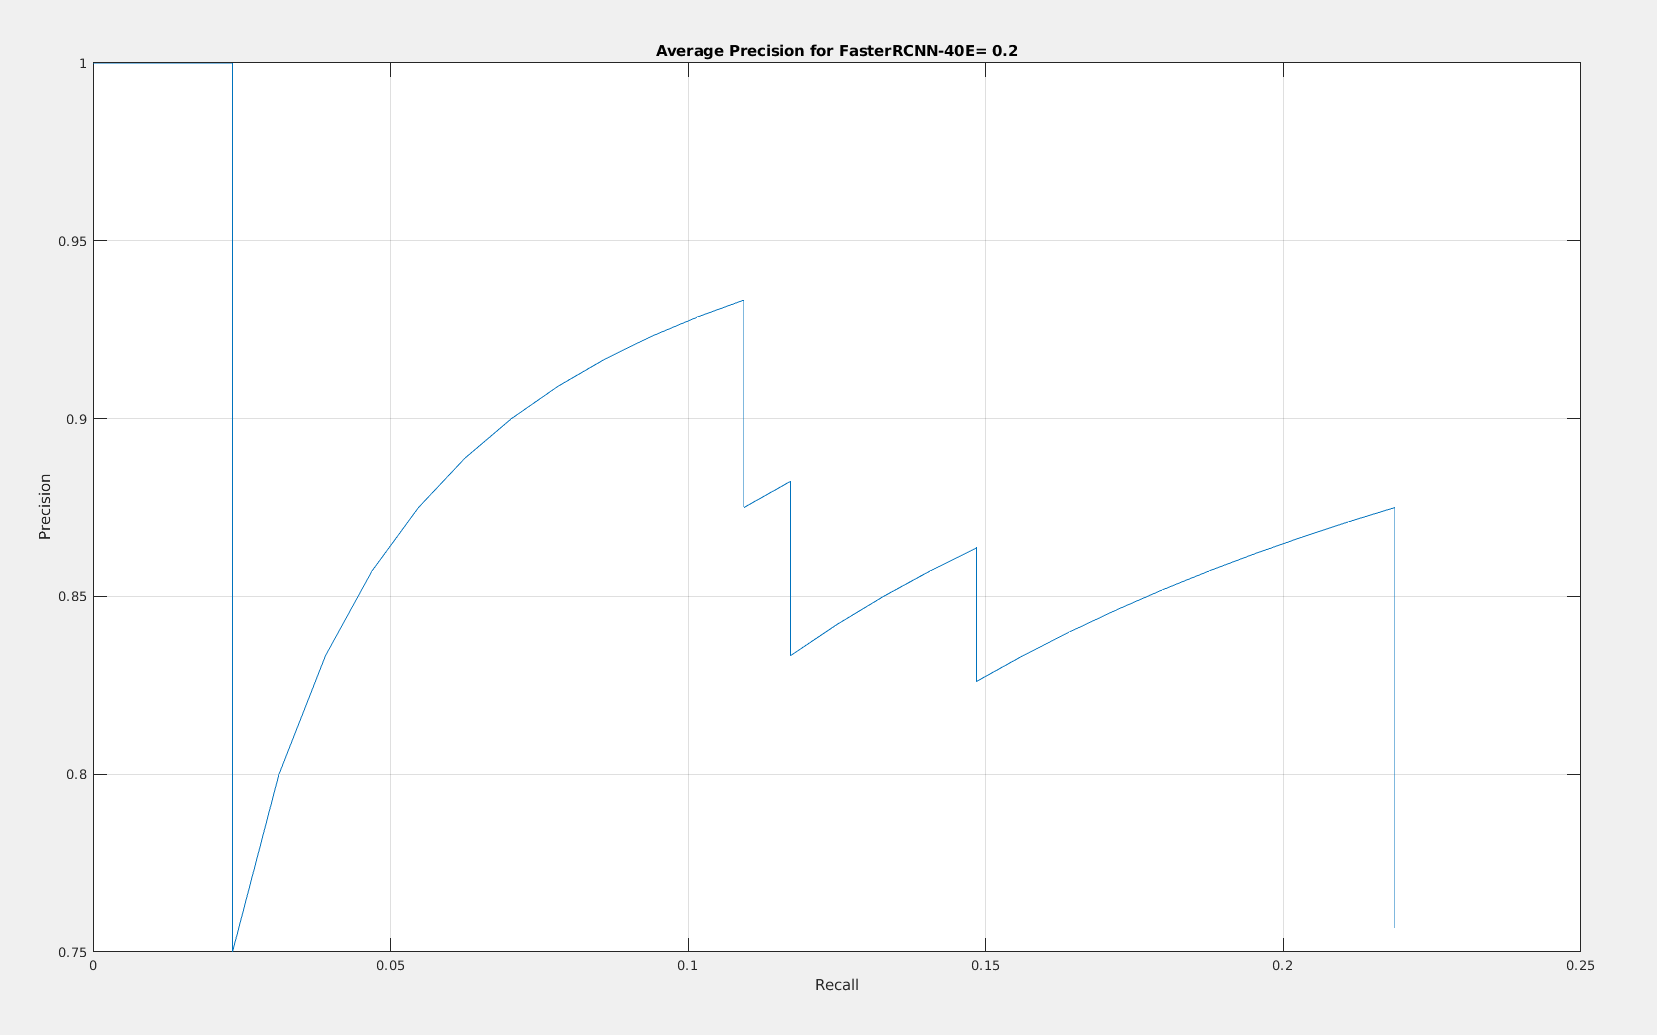
\includegraphics[width=12cm, height=5cm]{images/EvalRCNN40E.png} \\
         \space\textbf{ACF detector - trained in 5 steps}\\
         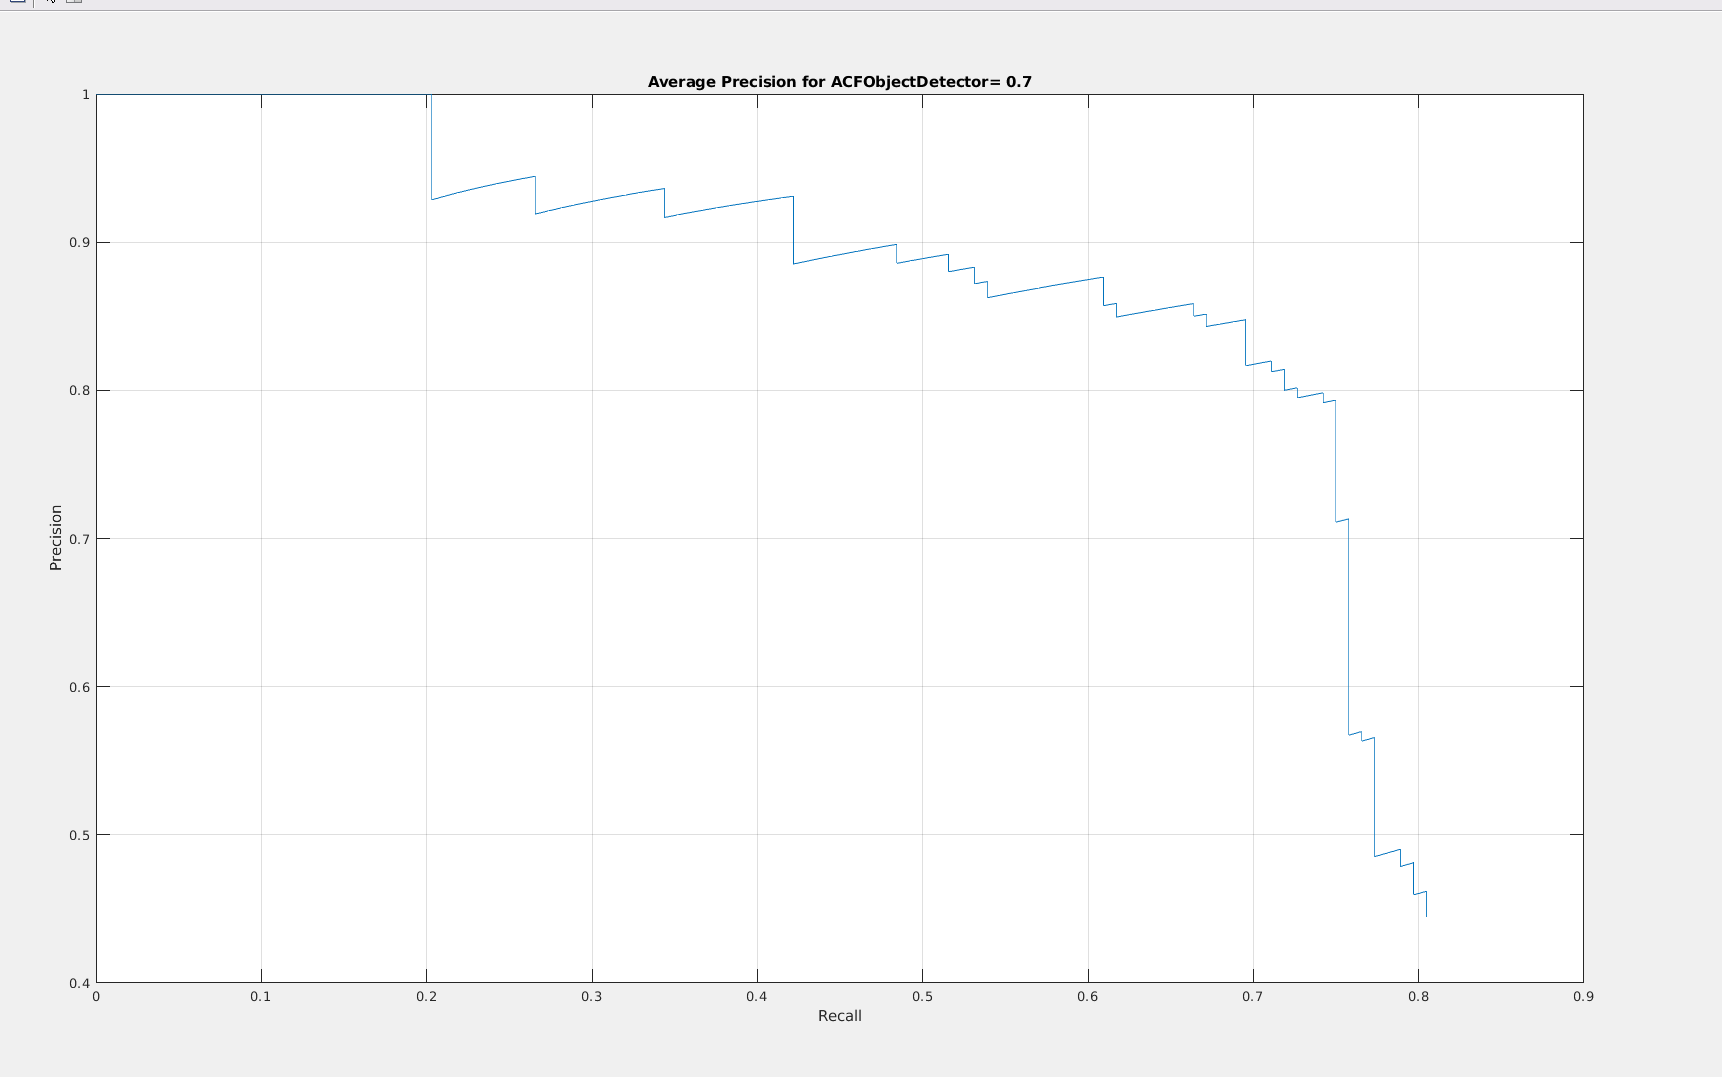
\includegraphics[width=12cm, height=5cm]{images/EvalACF.png}
    \end{tabular}
    \caption{Evaluation results of 3 detectors}
    \label{fig:evaluation}
\end{figure}

\section{Detection of Parking Vacancy}
After finding detected vehicles, next step is to find parking vacancy or an empty space between two adjacent vehicles which is perfect for parking. As already mentioned above, most of the defined methods like \cite{markingPointConf} depends on marking lines provided by parking-lots. However, as our environment was on a street which did not offer these line marking or any sign near parking places. Besides, the scenario is to find a parking vacancy and implement maneuver in the street not a garage with ordered lanes and signs to guide drivers to parking-places. In parallel parking in a random place on the street, there is always these problems that line markers in most places are too small and difficult to observe so it would be difficult to detect them by computer and most of the streets does not even have these markers for parking. In other words, city streets are full of line marks as traffic line, crossroads or lane dividers which would be difficult to separate them from parking lanes so most of the previous works in vision-based did not help to find a place of parking. The only thing we had in this project was bounding-boxes which provided by vehicle detection algorithm(ACF). Bounding boxes are the boxes highlights detected vehicles as it could be also seen in detected photos in fig \ref{fig:rcnnVsACFResult} and they provides us pixel coordinates of each detected car and each of them has a form of [x, y, width, height]. As it can be seen again in fig \ref{fig:rcnnVsACFResult} bboxes in each frame of detection, have partially overlapped and these overlaps could be used to find empty space between vehicles. If two vehicles has a high overlap ratio, it can be concluded that they are so closed together and the distance between them is very small so it would not be possible to park another car between them and vise versa. Hence, the idea is to measure how much two vicinity objects are overlapped. In this work IOU(Intersection Over Union)has been used to find overlap ratio of the boxes. IOU is a common measurement in computer vision and most of the detection algorithms have libraries to implement it. IOU can be defined by equation \ref{eq1} and it can be measured by the amount of pixels where two objects overlap dividing to the amount of pixels covered by both objects.
\begin{equation} \label{eq1}
\begin{split}
Intersection Over Union = \frac{Intersection of Boxes}{Union of Boxes}
\end{split}
\end{equation}
Overlap ratio will give us how much a car's bounding box overlaps with other car's bounding boxes i,e if this ratio is lower than 0.15, this means that their overlap is so small and there is a parking space between them but if this overlap is high (like more than 0.2) it means that the space between two vehicle is not big enough to place another car. However, we did not make parking decision just based on ratio data and after estimation of parking space and the probability of empty place, sensors are used to measure the exact distances between two vehicles(by low overlap rates). so this ratio gives us the likelihood of parking vacancy and is not the final decision. a detailed explanation about the sensors and how ego vehicles sets to the starting point of maneuver, has been provided in chapter \ref{chapter: stabilization}.

